% !TEX root = ./Thesis.tex

\chapter{Parahydrogen induced polarisation} \label{Chapter:Parahydrogen}

 The majority of the work in this chapter appears in \citep{eills2019high}

\section{Abstract}
In this chapter a device that combines high-resolution NMR and parahydrogen induced hyperolarization (PHIP)
with a high-sensitivity transmission line micro-detector is discussed.
The para-enriched hydrogen gas is introduced into solution by diffusion
through a membrane integrated into a microfluiduc chip.
NMR microdetectors, operating with sample volumes of a few $\mu$l or less,
benefit from a favourable scaling of mass sensitivity discussed
in \ref{Micro-NMR}. However, the small volumes make it very difficult to
detect species present at less
than millimolar concentrations in microfluidic NMR systems.

In view of
overcoming this limitation, parahydrogen-induced polarisation
(PHIP) is implemented on a microfluidic device with 2.5~$\mu$l detection volume.
Integrating the hydrogenation reaction into the chip minimises polarisation
losses to spin-lattice relaxation, allowing the detection of picomoles of
substance. This corresponds to a concentration limit of detection of better than
1$\mu$M$\sqrt{\text{s}}$, unprecedented at this sample volume.  The
stability and sensitivity of the  system can be used to extract
quantitative information on the hydrogenation kinetics and
their interplay with nuclear relaxation. It is further exemplified by homo-
(\textsuperscript{1}H-\textsuperscript{1}H) and heteronuclear
(\textsuperscript{1}H-\textsuperscript{13}C) 2D NMR experiments
 at natural \textsuperscript{13}C abundance.

 \section{Hyperpolarisation}


 \subsection{Sensitivity}\label{Sensitivity}

 In \ref{Population} it is demonstrated how NMR has low polarisation levels governed by the Boltzmann
 distribution given in \eqn{eqn:Boltzmann}. For example, for a spin-1/2 particle in a static field of 14.1 Tesla
 there is only a factor of $~6\times10^{-6}$ difference in the populations of the $\alpha$ and $\beta$ state.
 Compared to other spectroscopic techniques NMR suffers from poor limits of detection (LODs). Raman Spectroscopy, has
 LODs of $10^{-12}$ - $10^{-15}$, Laser indced flourescence (LIF) has detected concentrations at $10^{-13}$ and
 mass spectrometry has achieved $10^{-19}$. All of which are several orders of magnitude higher than that of NMR. While sensitivity is not a strong point, NMR is quantitaive, non-invasive, and non-destructive making it an ideal tool for mass limited or living samples.

 \subsection{Signal Averaging}\label{Signal Averaging}

 In NMR, the total signal that emerges from the probe contains signal from the sample
 under observation as well as uncontrolled random signals called noise. The most dominant source of noise comes from the thermal motions of the electrons
 in the receiver coil. In order for the signal that originated from the sample to rise above the noise,
 signal averaging must be employed. This works as the sum of two identical experiments is twice the signal
 of the orginal individual experiment:
 \begin{equation}
   s_\text{NMR}(1+2) = s_\text{NMR}(1) + s_\text{NMR}(2) = 2s_\text{NMR}(1)
 \end{equation}
 The key is that this relationship doesn't apply equally to the noise which as it is random. A suitable
 definition of the noise amplitude in a single experiment is given by the root mean square (RMS) noise defined
 as:
 \begin{equation}
   \sigma_\text{noise} = \langle~s_{\text{noise}}(1)^2\rangle^{1/2}
 \end{equation}
 where the angle bracket indicates an average over all sampling points. The RMS noise is the same for two
 experiments assuming the noise is stationary i.e. the noise doesn't change from one experiment to the next.
 However this does not imply that the noise from two experiments has twice the value. Summed over the two experiments
 the RMS noise takes the value:
 \begin{equation}
   \sigma_\text{noise}(1+2) \cong \sqrt{2} \sigma_{\text{noise}}(1)
 \end{equation}
 Since the noise over two experiments increases by $\sqrt{2}$ but the signal doubles. Therefore the signal to noise
 ratio over two experiments can be written as:
 \begin{equation}
   \text{SNR}(1+2) = \sqrt{2}\frac{s_{\text{NMR}}(1)}{\sigma_{\text{noise}}(1)}
 \end{equation}
 This can be extended to show the signal-to-noise over $N$ transients is a factor $\sqrt{N}$ larger than the
 signal for a single transient. So by signal averaging over many scans the SNR can be increased.

  In principle this allows NMR signals that have a SNR less than one to be 'pulled out' of the noise. In reality this is
  time consuming as in order to repeat an experiment precisely it is essential to allow the spin sytem to
  reach thermal equilibrium again. The different NMR experiments must therefore be separated by an interval
  many times longer than $T_1$, which in some case can be several seconds. For example, if the SNR of the first
  experiment is 0.1 clearly the signal will be buried in the noise. The SNR may be changed to 10:1 by signal averaging
  over 10,000 scans. If each scan takes 1 second this amounts to 3 hours of instrument time which is long but
  acceptable. However, if the SNR is 0.01 then it follows that 300 hours would now be needed which is not feasible.

  In order for smaller signals to be detected, the amount of signal i.e. the amount of polarisation in the sample,
  needs to be increased this can be done by preparing the sample in a specific way and is referred to as
  'hyperpolarisation'.

\subsection{Hyperpolarisation - not sure on order here}

 As mentioned in \ref{Sensitivity} the polarisation levels of nuclear spins at room tempersture is low. In fact,
 for protons it is only $3\times10{^-6}$ per tesla\citep{RN138}. The signal derived from an NMR experiment
 is proportional to this polarisation and means that the sensitivty and LOD is limited. The highest
 field avaiable commercially is ~28 Tesla which corresponds to polarisaiton levels in protons of ~$10^{-4}$ and
 whilst there are clear advantages to working in higher fields the size and more importantly - cost, make them unsuitable for many applications. Clearly just increasing the field is not a viable
 option if close to unity polarisation is to be
 acheived.

 There are techniques for increasing the spin polarisation levels in samples to beyond the thermal
 equilibrium. The general term used to describe these is hyperpolarisation. Hyperpolarisation has
 applications in a diverse range of fields such as MRI \citep{RN139,RN140,RN151,RN152}, drug discovery
 \citep{RN141,RN142}, reaction monitoring \citep{RN143,RN144,RN145}, metabolomics \citep{RN147,RN148},
 catalysis\citep{RN149, RN150} and material chemistry \citep{RN153,piveteau2015structure,RN154}.

 However, these hyperpolarised states are still subject to relaxation as discussed in \ref{Relaxation} and
 return to thermal equilibrium with time constant $T_1$. This means the hyperpolarised spin order lasts seconds
 to minutes which limits their applications.

 \subsection{Techniques}

 \subsubsection{Brute Force}

 The most simple technique for hyperpolarisation is "brute force". It is performed by simply
 cooling the sample to a few degrees kelvin in a high magnetic field \citep{RN155,RN157}. Under
 these circumstances the polarisation of the nuclei is ~$1\%$. After sufficient time has passed
 the sample is rapidly dissolved in a warm solvent in order to liberate the hyperpolarised
 species as a solution for detection.

 There are drawbacks however, firstly, long $T_1$ times at cryogenic temperatures means long
 wait times are required in order to sufficiently build up polarisation in the sample. Secondly, and
 perhaps more importantly, the limit of polarisation with this technique is around $10^{-2}$ at acheivable
 magnetic fields and temperatures.

 \subsubsection{Dynamic Nuclear Polarisation}

 Several different types of dynamic nuclear polarisation (DNP) have been reported. These are solution
 state DNP\citep{RN158}, solid state magic angle spinning (MAS) DNP\citep{RN159} and static solid state DNP with
 dissolution and observation\citep{RN160}. The latter is most commonly referred to as dissolution-DNP and written as d-DNP.

 DNP methods use the thermal equilibrium electron spin polarisation to polarize the nuclei under investigation. Unity
 polarisation of the electrons is achieved by cooling to cryogenic temperatures (<2K) in a high magnetic field (>7 T).
 The electron polarization is transferred to nearby nuclear spins by saturating microwave frequency radiation.

  The source of the electrons are 'free radicals' - molecules that have an unpaired elctron spin, that
  are spread homogeneously throughout the sample after cooling the sample is held in a cryostat which is at
  1.2 - 1.5K. The electrons have a much shorter $T_1$ in contrast to nuclear spins so after irradiation with
  microwave radiation to induce polarization transfer between elctrons and nuclei, the electrons repolarise
  quickly compared to the nuclei who retain non-equilibrium polarization. This polarization diffuses throughout the
  sample. After some time, tens of minutes is not uncommon, the nuclear spins are polarised to around 0.1. The
  sample is then rapidly dissolved with a pressurised hot solvent into a separate high field magnet for detection.

  The large equipment required for d-DNP, as well as the high cost of liquid helium for the cryostat and
  the superconducting magnets make this method  prohibitive for most NMR groups.

 \section{Parahydrogen Iduced Polarisation - PHIP}

 \subsection{Parahydrogen}

 Hydrogen exists as a diatomic made up of two protons and two electrons. As such, the total
 wave function contains electronic, vibrational, rotational and spin components and can be
 written as:

 \begin{equation}
  \Psi^{tot} =\Psi^{elec}\Psi^{vib}\Psi^{rot}\Psi^{spin}
 \end{equation}

 Because the two protons are fermions they are subject to the Pauli exclusion principle
 which states that the total wave function must be antisymmetric with respect to exchange. With
 this is mind, it is important to note that the electronic and vibrational states are symmetrical in the ground state and if we assume that they occupy the ground state, we find that the symmetry of the overall wave function depends of the symmetry of $\Psi^{rot}$$\Psi^{spin}$.

 Rotational wavefunctions have quantum number J. For even numbers of $J$ (J=0,2...) the wavefunction is symmetric with respect to particle exchange for odd numbers of J (J=1,3...) the wavefunction is antisymmetric. The nuclear spin wave function can also be symmetric or antisymmetric. By adding the angular momentum of both spins it can be shown that they combine to give four possible wavefunctions:


 \begin{align}
 \Psi_{1}^{T+} =& \ket{\alpha\alpha}\\
 \Psi_{1}^{T0} =& \frac{1}{\sqrt{2}} (\ket{\alpha\beta}+\ket{\beta\alpha})\\
 \Psi_{1}^{T-} =& \ket{\beta\beta}\\
 \Psi_{0}^{S0} =& \frac{1}{\sqrt{2}} (\ket{\alpha\beta}-\ket{\beta\alpha}).
 \end{align}

 The three triplet ($T$) states have spin quantum number I = 1 and are symmetric with respect to spin exchange whilst
 the singlet ($S$) state has I = 0 and is antisymmetric. Hydrogen in the triplet state is refered to as \textit{ortho} and the
 singlet state is referred to as \textit{para}.

 In order for $\Psi^{tot}$ to be antisymmetric the antisymmetric rotational states are restricted to the symmetric (triplet) spin states whilst the symmetric rotational states are restricted to the antisymmetric (singlet) state.

 The rotational energy is given by $E_j = \frac{J(J+1)\hbar^2}{2I}$
 where I is the moment of inertia of the diatomic and is given by $I = \mu l^2$, where $\mu$ is the reduced mass,
 and $l$ is the internuclear distance.

 \begin{figure*}
   \begin{center}
   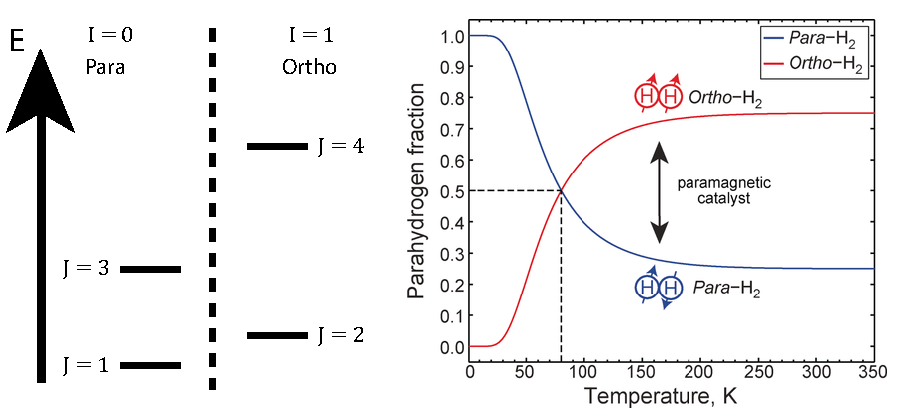
\includegraphics[width=\textwidth]{Para-OrthoH2.pdf}
   \end{center}
   \caption{Left: The rotational energy levels of para- and orthohydrogen with their associated J values. Right: a graph
   showing the fraction of para- and orthohydrogen as a function of temperature. The dotted line shows 50\% para
   enrichment that is acheived by cooling to 77K using liquid nitrogen. Image taken from \citep{barskiy2017nmr}.}
   \label{fig:POH2}
 \end{figure*}


 At room temperature the ratio of \textit{ortho} to \textit{para} hydrogen is 3 to 1. However, by cooling down hydrogen the lowest (J = 0, 1) rotational enrgy states start to become populated. By cooling alone the ratio would remain unchanged. One can't convert from ortho to para spin states without the aid of a catalyst (typically charcoal or iron (III) oxide). The catalyst temporarily breaks the symmetry of the \ce{H_2} molecule and allows these spin-spin transitions and allows a much larger fraction of the \textit{para} form of hydrogen to be produced. Crucially, when warmed up to
 room temperature in the absence of a symmetry breaking catalyst, no conversion from the singlet state $S_0$ back to
 the triplet states $T_+$, $T_0$, $T_-$ occurs. This is because the nuclear spin flip required would not
 conserve angular momentum and is therefore disallowed. It therefore possible to store pure parahydrogen
 in the right container for days to weeks.

 Para enrichment fraction, $f$, can be measured by NMR. By measuring the o\ce{H_2} signal of the enriched \ce{H_2} ($S_{e}$) and comparing it to the signal obtained from the same amount of \ce{H_2} at room temperature ($S_{rt}$). The enrichment fraction is given by[\citep{RN131, RN132}:

 \begin{equation}\label{pfrac}
   f = 1 -(3S_{e}/4S_{rt})
 \end{equation}

 \subsection{PASADENA and ALTADENA}\label{PASADENA and ALTADENA}

 Parahydrogen and synthesis allow dramatically enhanced nuclear alignment (PASADENA)\citep{RN129} and adiabatic longitudinal transport after dissociation engenders net alignment (ALTADENA)\citep{RN128}
  are subclasses of PHIP experiments characterised by the strength of magnetic
 field in which the hydrogenation and detection are performed.

 The difference between PASADENA and ALTADENA are the $J$-coupling regimes in which the reaction and detection happens. In PASADENA experiments the reaction and detection is carried out at high field (>1 T) whereas in
 ALTADENA, the reaction is carried out at low field (< 10 mT), and the product is transferred to a high magnetic field for detection\citep{RN130}.

 This difference manifests itself as a difference in $J$-coupling regimes in the \textit{para}hydrogen derived hydrogens in the product molecule. ALTADENA refers to hydrogens in the strong copupling regime and PASADENA refers to the weak cpoupling regime. The regime is determined by the value of the $J$-coupling (in Hz) compared to the value of the difference in chemical shifts of the individual protons.
 Where the strong regime has J-coulings that take the approxiamte value of the difference in chemical shift ($\frac{\delta{\omega}}{J}\approx1$) and the weak regime has J-couplings much smaller than the difference in chemical shift ($\frac{\delta{\omega}}{J}>>1$). Since the chemical shift depends on external magnetic field ($B_{0}$) and the J-couplings are independent of field one can select an appropriate magnetic field for the desired experiment.

 \subsubsection{Spin Physics}

 The spin physics of these types of hydrogenative PHIP are
 accessible through the density operator formulism. In a PASADENA type experiment, parahydrogen is then added to molecule in high field forming a weakly coupled AX
 system of the type discussed in \ref{PASADENA and ALTADENA}. Due to the weak coupling, $\frac{\delta{\omega}}{J}>>1$, the eigenbasis is close to the Zeeman basis. The initial density operator, $\hat{\rho}_{\text{ini}}$ from our earlier
 definitions this is:
 \begin{equation}
   \hat{\rho}_{\text{ini}} = \ket{\Psi_{0}^{S}}\bra{\Psi_{0}^{S}} = \frac{1}{2}\ket{\alpha\beta -
   \beta\alpha}\bra{\alpha\beta - \beta\alpha}
 \end{equation}

 using the zeeman basis states for a 2 spins system described in \ref{SpinStates}

 \begin{align}
   \hat{\rho}_{\text{ini}}\quad=& \frac{1}{2} \begin{pmatrix}
   0\\
   1\\
   -1\\
   0
   \end{pmatrix} \otimes \begin{pmatrix}
     0 & 1 & -1 & 0
     \end{pmatrix}\\
   =& \frac{1}{2}\begin{pmatrix}
   0 & 0 & 0 & 0\\
   0 & 1 & -1 & 0\\
   0 & -1 & 1 & 0\\
   0 & 0 & 0 & 0
 \end{pmatrix} \\
 \end{align}

 These diagonal elements (populations) do not evolve as these components commute with the Hamiltonian. The off-diagonal
 elements (coherences) evolve at a rate $\approx\delta{v}$.

 As the reaction continues an ensemble of molecules that are hydrogenated at different time points, this gives
 a new density operator, $\hat{\rho}_pr$, expressed as:
 \begin{equation}
   \hat{\rho}_{\text{pas}} = \frac{1}{t} \int_t=0^t{\text{exp}\{-i\hat{H}t\}\hat{\rho}_{\text{ini}}\text{exp}\{+i\hat{H}t\}}dt
 \end{equation}
 Usually, the hydrogenation period is much longer than the coherence evolution. These average to zero and so the
 density operator becomes:
 \begin{equation}
   \hat{\rho}_{\text{pas}} = \frac{1}{2}\begin{pmatrix}
   0 & 0 & 0 & 0\\
   0 & 1 & 0 & 0\\
   0 & 0 & 1 & 0\\
   0 & 0 & 0 & 0
 \end{pmatrix}
 \end{equation}

 \fig{fig:PASADENA} shows the eigenstate populations and general simulated spectra of a thermal equilibrium experiment and
 a PASADENA experiment.

 In a usual NMR spectra a $\pi/2$ pulse is used to excite observable single quantum coherences. For a PASADENA signal to
 be observed, a $\frac{\pi}{4}$ pulse must be used. The reason becomes clear when $\hat{\rho}_{\text{pr}}$ is rewritten
 in terms of angular momentum operators, neglecting the identity matrix this is:
 \begin{equation}
   \hat{\rho}_{\text{pas}} = -\hat{I}_{1z}\hat{I}_{2z}
 \end{equation}
 a $\frac{\pi}{2}$ pulse has the following effect:
 \begin{equation}
   \hat{\hat{R}}_y(\frac{\pi}{2})\hat{\rho}_{\text{pas}} = -\hat{I}_{1x}\hat{I}_{2x}
 \end{equation}

 which is an unobservable double quantum cohenrence and the reason pure parahydrogen is NMR silent. However,
 a $\pi/4$ $y$-pulse gives:
 \begin{equation}
 \hat{\hat{R}}_y(\frac{\pi}{4})\hat{\rho}_{\text{pas}} = -\frac{1}{2}(\hat{I}_{1x}\hat{I}_{2x} + \hat{I}_{1x}\hat{I}_{2z} + \hat{I}_{1z}\hat{I}_{2x} + \hat{I}_{1z}\hat{I}_{2z})
 \end{equation}
where the $\hat{I}_{1x}\hat{I}_{2z}$ and $\hat{I}_{1z}\hat{I}_{2x}$ terms are observable.
 \begin{figure*}
   \begin{center}
   \includegraphics[width=0.7\columnwidth,height=7cm,keepaspectratio]{Pasadena-population-Balls.pdf}
   \end{center}
   \caption{Above: Populations of states represented as balls in a thermal (left) and a PASADENA experiment. Below: Simulations of spectra arising from adding thermal hydrogen to a molecule (left) and of a PASADENA experiment when adding parahydrogen.}
   \label{fig:PASADENA}
 \end{figure*}

 In an ALTADENA exeriment, the hydrogenation is performed at low field. In this case, when a molecule of hydrogen
 is added to a substrate the denstiy operator - $\hat{\rho}_\text{ini}$, is projected onto the new eigenbasis which
 at low field (where $\frac{\delta{\omega}}{J}<<1$) is the singlet-triplet basis. To a good approximation the only term is the $\ket{S_0}$ and there is no evolution of the system.

 The sample is then transferred to high-field (where $\frac{\delta{\omega}}{J}>>1$). It is done adiabatically, this is defined as the rate of change of magnetic field being small with respect to the value of the $J$-coupling between them, squared denoted as $(J_{12})^2$. As the field increases, the eigenbasis changes from singlet-triplet to the Zeeman basis. The adiabatic change carries the population of the $\ket{S_0}$ state to the $\ket{\alpha\beta}$ state this is shown graphically in \fig{fig:SingletTriplet} In this case, only one of the four energy levels, namely $\alpha\beta$ is now populated, therefore the density operator, $\hat{\rho}_{alta}$ is given by:
 \begin{equation}
   \hat{\rho}_{\text{alta}} = \ket{\alpha\beta}\bra{\alpha\beta}
 \end{equation}
  This leads to \citep{RN128}:
 \begin{equation}
   \hat{\rho}_{\text{alta}} = \hat{I}_{1z}\hat{I}_{2z}±(\hat{I}_{1z}-\hat{I}_{2z})
 \end{equation}

 \begin{figure}
   \begin{center}
   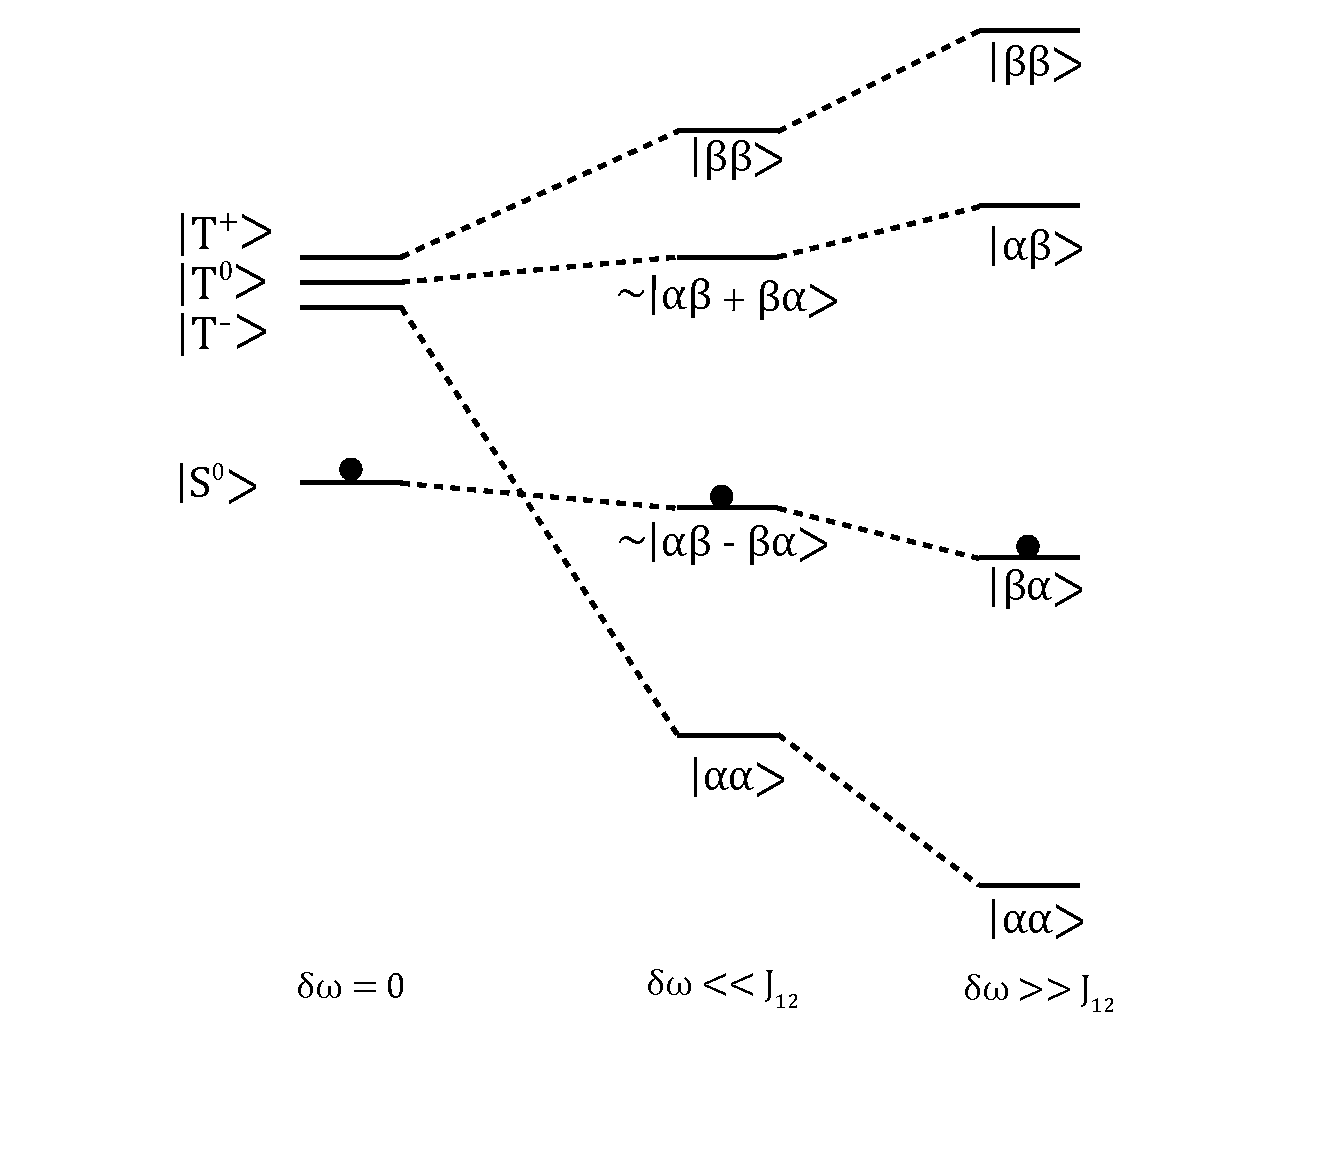
\includegraphics[width=0.7\columnwidth,height=7cm,keepaspectratio]{ALTADENA-overview.pdf}
   \end{center}
   \caption{Correlation diagram for the ALTADENA effect. Hydrogenation at low field populates the singlet state, adiabatically icreasing the field carries the population into a high field state.}
   \label{fig:SingletTriplet}
 \end{figure}

 The result of a $\pi/4$ pulse along the $y$-axis yields:
 \begin{equation}
   \hat{\hat{R}}_y(\frac{\pi}{2})\hat{\rho}_{\text{alta}} = \frac{1}{2}(\hat{I}_{1z}\hat{I}_{2x})±\frac{1}{2\sqrt{2}}(\hat{I}_{1x}-\hat{I}_{2x})
 \end{equation}
 This gives rise to the two out of phase doublets that are typical for an ALTADENA experiment on an AX system. A diagram
 is provided in \fig{fig:ALTADENA} that shows a simulated spectra compared to a thermal spectrum.

 \begin{figure}
   \begin{center}
   \includegraphics[width=\columnwidth,height=7cm,keepaspectratio]{Altadena-Population-Balls.pdf}
   \end{center}
   \caption{Top: Populations of Zeeman states represented by balls for thermal(left) and ALTADENA(right) experiments.
   Bottom: Simulations of a thermal spectrum after applying a $\pi/4$ pulse and an ALTADENA experiment.}
   \label{fig:ALTADENA}
 \end{figure}



\section{Introduction}

\begin{figure*}
  \centering
  \includegraphics[width=15cm]{mu1y11-ph2c-fi-190511-paa-reaction-scheme.pdf}
  \caption{
    Scheme of the reaction used in the PHIP@chip experiment. Hydrogen gas
    \textbf{1}
    enriched in parahydrogen reacts with propargyl acetate \textbf{2} in
    the presence of the Rh catalyst \textbf{3} to form allyl acetate \textbf{4}.
  }
  \label{fig:reaction-scheme}
\end{figure*}

\begin{figure}
	\centering
	\includegraphics[width=7cm]{mu1y11-ph2c-fi-190117-fig1.png}
	\caption{Overview of the PHIP@chip device.
		% a: scheme of the hydrogenation reaction;
    %
    a: outline drawing of the chip (dimensions in mm).
		b: CAD rendering of the chip assembly with individual chip layers
		separated, consisting of the PMMA chip, PDMS membrane, and two 3D
		printed holders with threads for the gas and fluid connections.
    The hydrogen gas
		diffuses through the PDMS membrane into the flowing liquid.
		}
	\label{fig:phip@chip1}
\end{figure}

High-resolution NMR
spectroscopy is a superbly versatile method which provides detailed and
quantitative information on chemical composition and structure. It is widely
used to follow the progress of chemical reactions
\cite{Foley-quantitative:2004bk,Foley:2014kpa},
as well as
metabolic processes in living systems
\cite{Wishart:2008ga,Gottschalk:2008ixa,CuperlovicCulf:2010vc,Shintu:2012bl}.
However, NMR suffers from inherently low sensitivity,
which is due in part to the very weak polarisation of nuclear spins along the magnetic
field for samples in thermal equilibrium at ambient conditions.
Conventional high-resolution NMR therefore requires nanomole quantities of
sample. Many important problems require detection of analytes at low
micromolar concentrations, such as transient reaction intermediates, or
metabolic species. Despite the
comparatively higher mass sensitivity of NMR for small sample volumes
\cite{Olson:1995vu,Bart:2009kc}, conventional micro-NMR systems  around
1~$\mathrm{\mu l}$ achieve mass limits of detection of no better than\cite{Finch:2016gv}
1~nmol$\sqrt{\mathrm{s}}$,  corresponding to a concentration
limit of detection of 1~$\mathrm{m M \, \sqrt{s}}$. An increase of several
orders of magnitude in sensitivity is therefore be required to enable NMR
studies of mass-limited samples at micromolar concentrations.

Microfluidic lab-on-a-chip devices are finding increasing applications in
chemistry and the
life sciences. They provide detailed control over the experimental
conditions at a much smaller length scale than conventional reactors, and
allow integration of synthesis, separation, and analytical steps on
a single platform \cite{Wang:2006en,Theberge:2012iq,Hoang:2011du,Ohno:2008da,Zhou:2004id,
Fang:2018ib,Hoang:2011ee,Gunther:2006vd}. The small size also affords the possibility of
high experimental throughput.
In the life sciences, microfluidic devices are increasingly used as
sophisticated culture platforms for cells,
cell assemblies, tissues, and small organisms
\cite{Manz:1990vc,Whitesides:2006vi,
ElAli:2006ci,West:2008jd,Neuzil:2012gc,Gracz:2015co}.
The integration of NMR with microfluidics
\cite{Ryan:2012ke,Badilita:2011td,Spengler:2014ir,Finch:2016gv} is promising, as
it enables in-situ, non-invasive monitoring of chemical and metabolic processes
in lab-on-a-chip systems.

The usefulness of microfluidic NMR could therefore be significantly
enhanced if the following conditions could be met:
(i) sample volumes around 1~$\mu$l or less;
(ii) a concentration limit of
detection near  1~$\mu$M$\sqrt{s}$; and
(iii)  spectral
resolution of better than 0.01~ppm to allow distinction and identification
of chemical species.

Although exquisitely sensitive NMR detection schemes exist,
approaching even single-spin detection in favourable cases
\cite{Rugar:1992dm,Rugar:2004bc,Mamin:2007ff,Poggio:2010jf,
Maze:2008cs,Staudacher:2013kn,Rugar:2015by,McDermott:2002hp,
Budker:2007hz,Xu:2006kg,Blanchard:2013gs}, they lack spectral resolution.
While a recent study
has demonstrated resolution of $J$ couplings using a nitrogen-vacancy
(NV) centre magnetometer.\cite{Glenn:2018ct}, none of these
alternative detection schemes are compatible with high (several Tesla)
magnetic fields, which are essential to produce spectral dispersion
by chemical shifts.
So far, no method has been demonstrated with the combination of high
spectral resolution, high chemical dispersion,
and high sensitivity for small volumes required for
advanced microfluidic NMR measurements significantly
below the 1~mM concentration scale.

Hyperpolarisation methods generate substances which exhibit a transiently high
level of nuclear spin polarisation, with an increase in the NMR signal strength
of more than 4 orders of magnitude \cite{munnemann2011nuclear}, can be combined
with micro-NMR detectors and microfluidic systems \cite{McDonnell:2005dn,Desvaux:2009bq,Telkki:2010vg,Paciok:2011ek,JimenezMartinez:2014et,Causier:2015fg,eills-hale2018EuromarPHIP,Bordonali:2019jqa}.
One such method
involves the chemical reaction of the singlet spin isomer of molecular
hydrogen, and is called parahydrogen-induced hyperpolarisation (PHIP)
\cite{hovener2018parahydrogen,duckett2012application,gloggler2013hydrogen,green2012theory}.

While most studies have so far brought the reaction liquid in direct contact
with hydrogen gas either through bubbling or by atomisation of the liquid
in a hydrogen-filled chamber \cite{bhattacharya2007towards,chekmenev2008pasadena,
chekmenev2009hyperpolarized,shchepin2014parahydrogen,
Reineri:2015he,cavallari201813,eills2017singlet},
liquid-gas interfaces and in particular bubbles
pose difficulties in the context of microfluidic devices, since they tend
to alter the flow properties, and can block fluid transport altogether.
Continuous delivery of parahydrogen by diffusion through
gas-permeable membranes has been demonstrated at
conventional size scales \cite{Roth:2010hk,Lehmkuhl:2018cd}.
It has been shown that silicone elastomer membranes can be used
to deliver parahydrogen directly to a flowing liquid in a microfluidic
device \cite{eills-hale2018EuromarPHIP}. Bordonali et al\cite{Bordonali:2019jqa} have
recently combined a microfluidic NMR probe system with a gas exchange
chip based on a silicone elastomer membrane to implement the SABRE (signal
enhancement by reversible exchange) variant of parahydrogen-induced polarisation,
but achieved only small signal enhancement factors (3 to 4).

In distinction from previous work
\cite{bhattacharya2007towards,chekmenev2008pasadena,
chekmenev2009hyperpolarized,shchepin2014parahydrogen,
Reineri:2015he,cavallari201813,eills2017singlet,Lehmkuhl:2018cd},
this work integrates the hydrogenation reactor into the chip itself, which greatly
reduces the polarisation losses due to spin-lattice relaxation.
As shown below, a signal enhancement factor over thermal polarisation
of about 1800 is achieved, allowing detection of a
picomole quantity of analyte in a sample volume of 2.5 $\mu$l,
while maintaining the full resolution of conventional $\ce{^1H}$
NMR spectroscopy.

This is accomplished by letting the parahydrogen gas diffuse through a
silicone elastomer membrane \cite{Lehmkuhl:2018cd}
to come into contact with a solution
flowing through the chip at a constant rate. The solution
contains a precursor, which is hydrogenated through a homogeneous
catalyst also present in the solution.
The microfluidic device is held in the bore of a conventional
NMR magnet using a purpose-built transmission line NMR probe.
This yields a continuous on-chip stream of hyperpolarised material. As shown
in the following, in addition to very high detection
sensitivities, this also results in a continuous and highly stable operation
of the system, making it possible to perform hyperpolarised
two-dimensional NMR experiments \cite{Roth:2010hk,Giraudeau:2009fn,Lloyd:2012cf,Eshuis:2015ce}.
By replacing the hyperpolarised gas feed with hydrogen gas at thermal
equilibrium, it is possible to gain kinetic information on the hydrogenation
process, as well as to calibrate the intensity of the hyperpolarised NMR signals.
This allows accurate assessment of the achieved polarisation levels, something
that has been notoriously difficult in the context of
parahydrogen-induced polarisation.


\section{Materials and methods}\label{pHMaterialandMethods}
The
microfluidic chips were constructed from three layers of cell cast PMMA sheet
material (Weatherall Equipment).  The sheet thickness was 200 $\mu$m for the
top and bottom layers, and 500 $\mu$m for the middle layer. The fluid and gas
channels were designed on AutoCAD and cut into the PMMA using a laser cutter
(HPC Laser L3040) to a width and depth of 150 $\mu$m. The layers were
subsequently bonded together with a plasticiser (2.5\% v/v dibutyl phthalate in
isopropyl alcohol) under heat and pressure (358 K, 3.5
tonnes) \cite{Yilmaz:2016fx}. The total internal fluid volume is 4~$\mu$l, and
the sample chamber is 2.5~$\mu$l.

The device also employs a poly(dimethyl siloxane) (PDMS) membrane
(Shielding Solutions) to facilitate para-H\textsubscript{2} transport,
of 1 mm thickness with laser-cut screw holes. The parahydrogen
polarisation lifetime in the PDMS after O\textsubscript{2} removal was
measured to be \textasciitilde{}4 h. To determine the hydrogen ortho- para
conversion in PDMS, the ortho-para conversion time of H2 dissolved in PDMS
was measured. A high-pressure NMR tube of 5 mm outer diameter
(Sigma-Aldrich) was filled with PDMS resin (Sylgard 84, 3M). A teflon
capillary of 1/16 inch outer diameter (Sigma-Aldrich) was pushed
into the NMR tube along the central axis, and the PDMS was allowed to cure.
The capillary was then removed, leaving a cylidrical void in the centre of
the NMR tube. The tube was then exposed to vacuum for varying amounts of
time, in order to study the conversion effect of the residual oxygen the
results of which are shown in \fig{fig:ph2conv}.

\begin{figure}
  \includegraphics[width=\columnwidth]{PDMS-Ts.png}
  \caption{Ortho-para conversion of hydrogen in PDMS after various times
  under vacuum.}
  \label{fig:ph2conv}
\end{figure}

The PMMA chip and PDMS membrane layer are sealed with a pair of
screw-tightened 3D printed (Accura Xtreme, Proto Labs) holders, with
fluid and gas in/out ports (to fit Kinesis UK NanoPorts).

The assembled microfluidic device was put in a transmission line based
home-built probe \cite{RN164}. The
device sits between the two stripline planes on a sample holder having
sample chamber of the device coinciding with the constriction on
stripline planes. All NMR experiments were performed at a field strength
of 11.7~T with an AVANCE III console. Nutation frequenies for RF pulses
were 100~kHz for protons, and 20~kHz for carbon in the case of the HMQC
spectrum. 16k data points were acquired over 1.2~s for proton 1D spectra.
Saturation recovery experiments used a train of 512 $\pi/2$ pulses
separated by a delay of 0.1~ms, followed by a recovery delay, and a $pi/4$
excitation pulse.
The PH-TOCSY spectrum was acquired using the States-TPPI method,
with 256 $t_1$ increments, averaging 8 transients per increment.
2048 complex data points in 0.2~s were acquired for each increment.
The PH-HMQC experiment was acquired using the States method, with
128 $t_1$ increments, averaging 8 transients with 2048 complex points
over 0.2~s. 1D spectra were processed using MestreNova (Mestrelab, Italy).
2D spectra were processed using scripts written in Julia \cite{Bezanson:2017gd}.

To generate parahydrogen gas at 50\% para enrichment, hydrogen gas
(purity 99.995\%) was passed through a home-built parahydrogen generator
containing an iron (III) oxide catalyst cooled to 77~K using liquid
nitrogen.

The solution before reaction contained 20 mM propargyl acetate \textbf{2}
and 5 mM
1,4-bis(diphenyl\-phosphino)\-butane(1,5-cyclo\-octadiene)\-rhodium
tetra\-fluoro\-borate \textbf{3} in methanol-d\textsubscript{4}. In an attempt to
avoid possible spin relaxation or chemical side-reaction effects,
dissolved oxygen from the atmosphere was removed by 5 minutes of
vigorous helium bubbling.

The parahydrogen gas was delivered through a PTFE tube (1/16 inch O.D.,
1/32 inch I.D.) into the 3D printed chip holder, and out via a second
PTFE line, using a mass flow controller (Cole-Parmer) to limit the flow
to 20 ml min\textsuperscript{-1} at an overpressure of 5 bar. Although
most of the parahydrogen gas passes directly through the system, some
amount dissolves into the PDMS layer, which in terms of
H\textsubscript{2} solubility behaves similarly to other organic
solvents. The solution was loaded into a 3.5 ml plastic syringe with a
Luer lock connection to in-flow PEEK tubing (1/16 inch O.D., 0.007 inch
I.D.) leading to the chip. The same tubing was used for the solution
out-flow into a container exposed to a back pressure of 1.5 bar of
nitrogen gas, to preventing formation of hydrogen bubbles in the chip.
Solution flow into the chip was controlled with a syringe pump (Cole-Parmer).

\section{Results and Discussion}
The hydrogenation reaction system employed in the present work is shown in
\fig{fig:reaction-scheme}.
Para\-hydrogen-en\-riched hydrogen gas $\mathbf{1}$ was
allowed to react with propargyl acetate $\mathbf{2}$, in the presence of
a rhodium catalyst $\mathbf{3}$. The substrate $\mathbf{2}$ was chosen in
view of future studies based on side-arm hydrogenation
\cite{Reineri:2015he,cavallari201813,cavallari2015effects}.

\subsection{ALTADENA}

In order to verify that the parahydrogen transfer on chip was possible, an
experiment was performed whereby the parahydrogen transfer was microfluidic
and ‘on chip’ but the detection was performed in a conventional NMR tube and probe.

This ALTADENA type experiment involved the addition of para enriched hydrogen
gas to propargyl acetate outside the magnetic field in a device shown in FIG. This device
is a simpler version of the one eventually used.
It features 3D printed holders that are used to deliver the gas and liquid as
well as seal against any liquid or gas leak. The chip is made from a single 500
$\mu$m thick layer of PMMA with serpentine paths for liquid and gas flow. B in the
\fig{fig:AltadenaChip} shows the path structure in the chip as well as the hydrogen and fluid paths
respectively.

\begin{figure}
  \begin{center}
  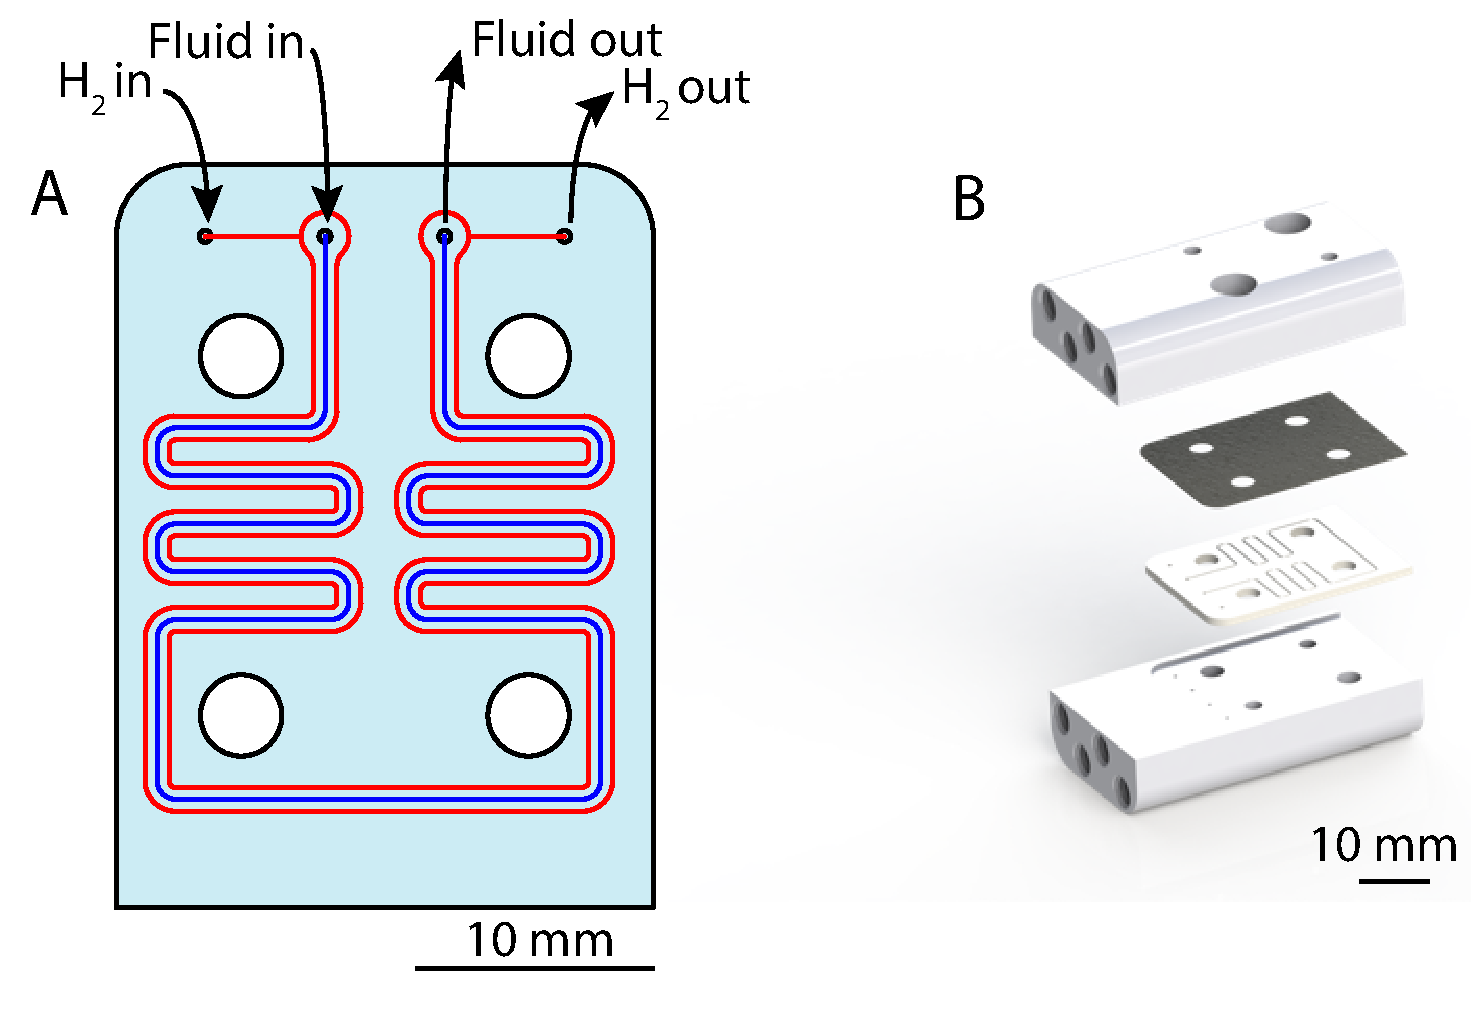
\includegraphics[width=\columnwidth]{ALTADENA-FIG.pdf}
  \end{center}
  \caption{A) Liquid channel (blue) and hydrogen channel (red) as scored
  onto the PMMA layer of the device. B) A 3D render of the hydrogenation device
  used for the ALTADENA experiements.}
  \label{fig:AltadenaChip}
\end{figure}

The set-up for this experiment employs a syringe pump, the hydrogenation device
outside the magnet and a standard 5 mm NMR tube inside the 16.5 T magnet. The device
was pressurised with 5 bar of 50\% enriched parahydrogen and allowed to equilibrate
for some time. Then, 100 $\mu$l was flown through the device at a flow rate of 1000
$\mu$l min$^{-1}$ this was done to ensure the sample from the experiment would reside
completely in the sensitive area. For the ALTADENA, 350 $\mu$l was flown through
the device and collected in the magnet. A $\pi$/4 pulse was applied and the spectra
recorded the result of the experiment is shown in \fig{fig:AltadenaResults}.

\begin{figure}
  \begin{center}
  \includegraphics[width=\columnwidth]{Altadena-Signal-comp.png}
  \end{center}
  \caption{Spectra obtained from i) a thermal hydrogenation and ii) a parahydrogenation
  of propargyl acetate to give allyl acetate with hydrogens derived from parahydrogen labelled a and
  b. By comparison of SNR the enhancement for the ALTADENA experiment is ~200. }
  \label{fig:AltadenaResults}
\end{figure}

A comparison is shown between scans taken of the same experiment, in \fig{fig:AltadenaResults} i) spectra
from an experiment with thermal hydrogen and ii) one with parahydrogen. The parahydrogen
ALTADENA signal (ii) exhibits the characteristic inverted peaks and a much higher signal
to noise ratio (SNR) and gives enhancement by comparison of the SNR of around 200.
This result proved that parahydrogenation induced polarisation (PHIP) on a chip
was possible by bubble free transfer through a PDMS membrane in our devices.

\subsection{PASADENA}

\begin{figure}
  \begin{center}
  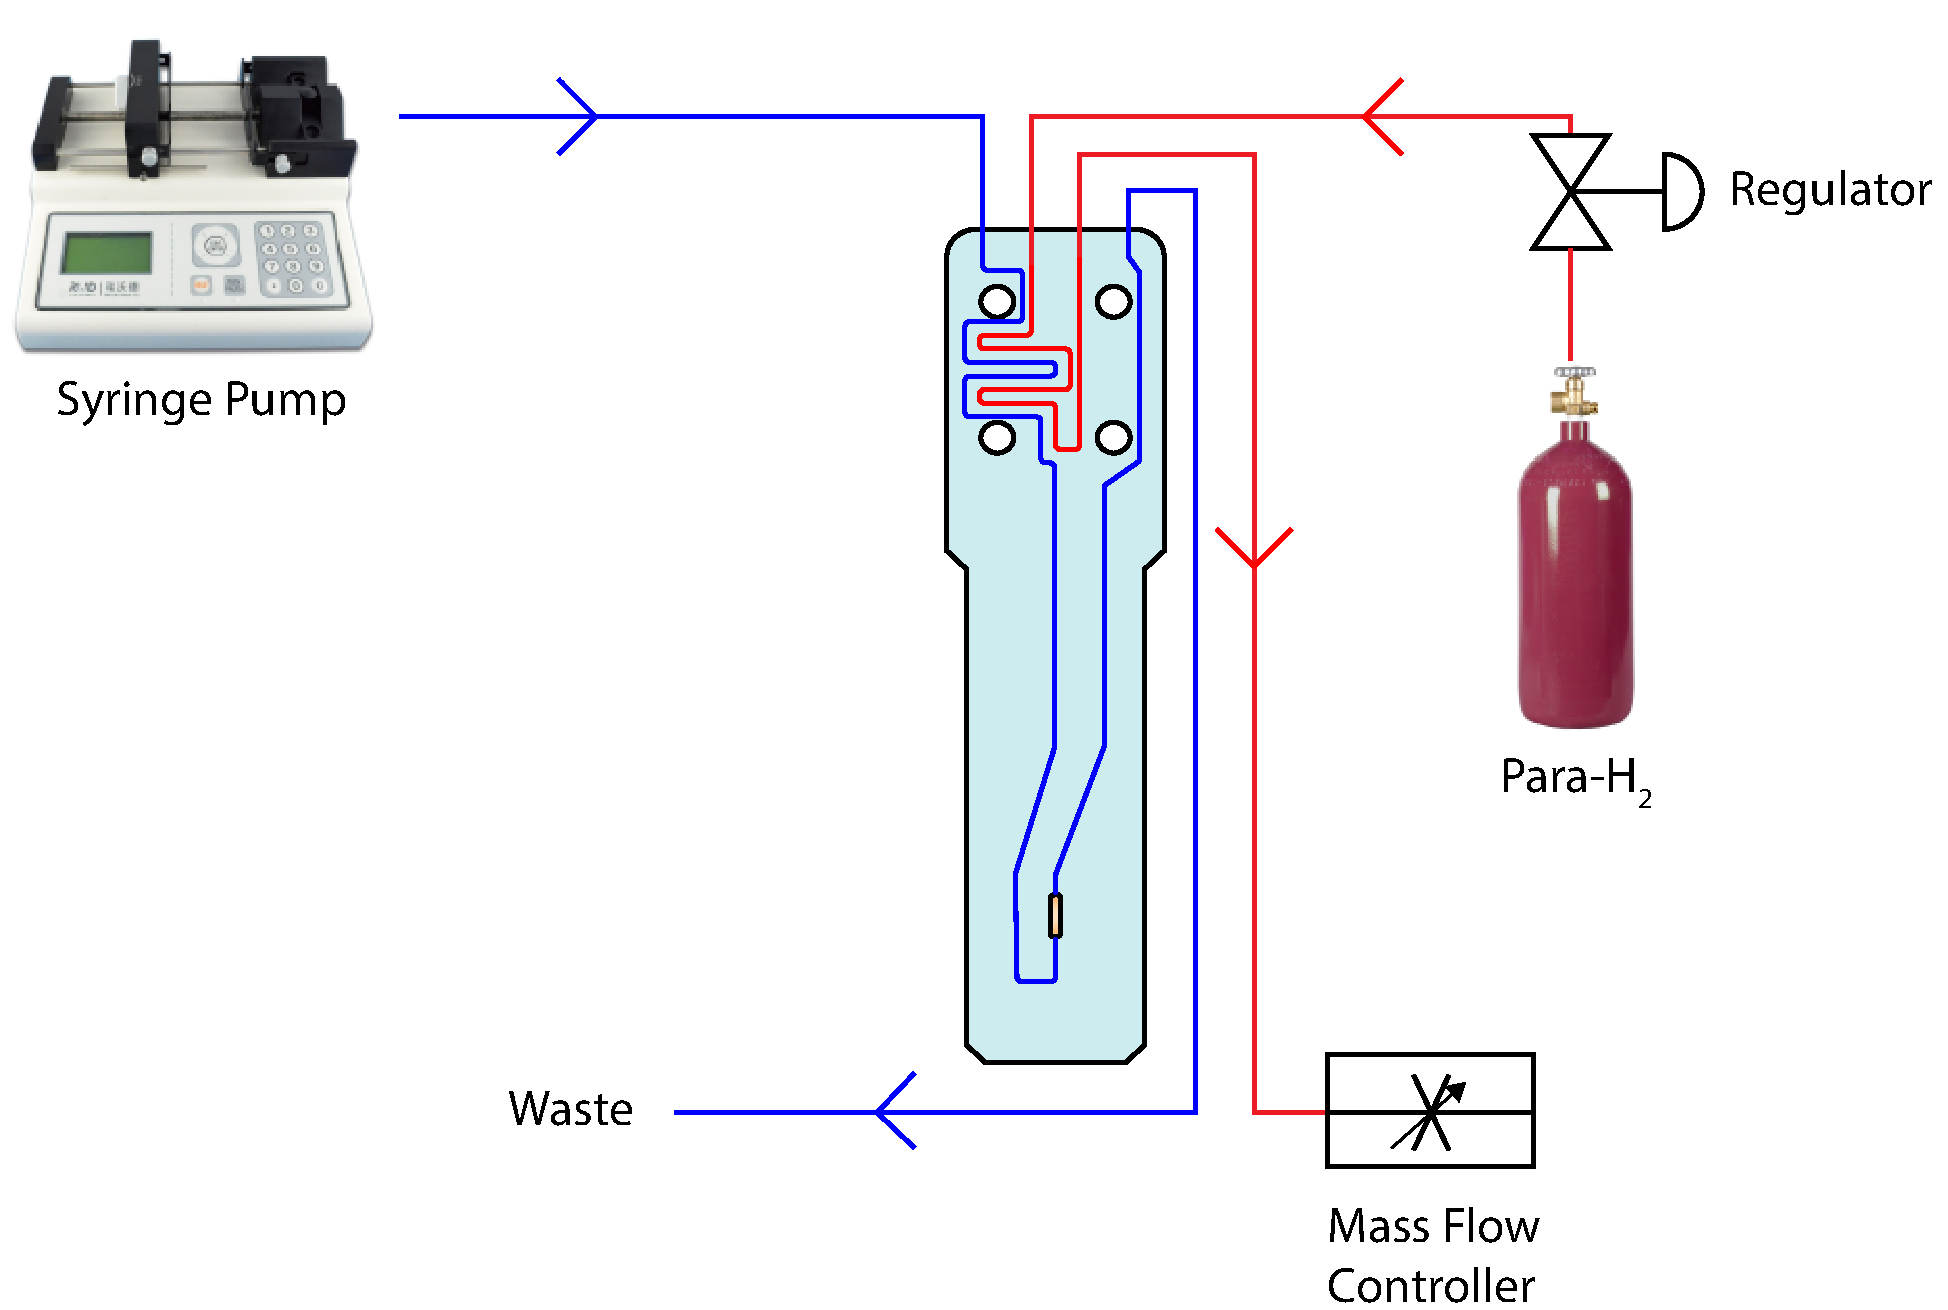
\includegraphics[width=\columnwidth]{PHIP-setup.pdf}
  \end{center}
  \caption{Drawing of PHIP@chip setup. It shows the solution (blue line)
  of propargyl acetate, catalyst and methanol being fed into the magnet
  via a syringe pump. Simultaneously, parahydrogen (red line) is fed in
  at the desired pressure and regulated by a mass flow controller to a
  flow rate of 20 ml$\text{min}^{-1}$. Both of these are fed into the
  microfluidic device depicted in \fig{fig:phip@chip1}}
  \label{fig:SetUp}
\end{figure}

\fig{fig:phip@chip1} shows the microfluidic device used for the
present study. It consists of a chip made from PMMA, which houses a sample
chamber of 2.5~$\mathrm{\mu L}$ volume that aligns with the transmission line
detector of a home-built NMR probe assembly, which was fitted inside of an
11.7~T NMR magnet.
Fluid is flowed through the chip by means of a syringe pump
installed outside of the magnet bore; connections are made through threaded
ports in the two 3D-printed holders shown in \fig{fig:phip@chip1}b.
Para-enriched H\textsubscript{2} gas at 5~bar above ambient pressure flows
through a second
channel in the chip, which runs in
the immediate vicinity of the liquid channel. A depiction of the set-up is given in \fig{fig:SetUp}.


\begin{figure}
	\centering
	\includegraphics[width=8cm]{mu1y11-ph2c-fi-100506-buildup-curve.pdf}
	%
	\caption{a: Single-scan proton NMR spectrum obtained with
  parahydrogen at 5 bar using the PHIP@chip setup at a continuous
  flow rate of 8~$\mu$L$\,\text{min}^{-1}$ (top trace with enlargement).
  Antiphase doublets from the two
	hyperpolarised protons $\mathrm{H}^a$  and $\mathrm{H}^{b}$ are
  clearly visible at 5.2~ppm and 5.9~ppm, respectively. Without
  parahydrogen, these signals are not observed (bottom trace).
	%%
	b: Buildup of the hyperpolarised signal ($\mathrm{H}^{a}$)
  after initiation of flow.
	%
	}
	\label{fig:phip@chip2}
\end{figure}


The chip consists of three laser-cut layers of poly methylmethacrylate (PMMA)
bonded together, as shown in \fig{fig:phip@chip1}b. Channels in the
left part of the chip, where it is clamped between the holders, are cut through
the top layer, while they are scored into the middle layer of the chip (and
hence sealed from the outside) in the free part of the device.
Within the clamps, the exposed channels are sealed by means of a PDMS membrane.
The flowing liquid as well as
the pressurised hydrogen gas are therefore exposed to the PDMS layer,
which serves as a diffusion bridge for the hydrogen.
The holders, made by 3D printing, keeps the membrane and the chip aligned,
and maintains mechanical pressure to ensure sealing. Channels
inside the holders guide the fluid and gas to and from
the four access points at the top end
of the chip, as shown in \fig{fig:phip@chip1}b.
The PDMS membrane acts both as a diffusion conduit for hydrogen gas
and as a fluid seal.
In a crucial difference to the otherwise similar geometry of the
hydrogenation chip used by Bordonali et al\cite{Bordonali:2019jq},
the gas and liquid channels are arranged side by side, and molecular
hydrogen diffuses through the bulk of the PDMS membrane rather than across the membrane. Clamping the PDMS membrane onto the chip using the
holders, makes it possible to use large gas pressures (up to 5 bar in
the present experiments). This would be difficult to achieve in the
chip presented by Bordonali et al, which has the liquid and gas channels
arranged on opposite sides of the membrane.

\subsection{Signal Analysis}

\fig{fig:phip@chip2}a shows a single-scan proton NMR spectrum
obtained from a steady-state PHIP@chip experiment (top trace), compared
to the spectrum obtained without parahydrogen (bottom trace).
The hyperpolarised spectrum is dominated by an antiphase doublet,
centred at 5.17~ppm, and an antiphase multiplet at 5.92~ppm, corresponding to
protons in the $\mathrm{H}^a$ and $\mathrm{H}^b$ positions of the
hydrogenation product \textbf{4}.
The PDMS membrane is equilibrated with para-enriched hydrogen gas, which is
supplied from an aluminium storage tank at a regulated pressure of 5~bar. The
gas flow rate is kept constant at 20~$\text{mL}\,\text{min}^{-1}$ by means of a
mass flow controller placed after the chip. This ensures that the gas channel
always contains fresh para-enriched hydrogen gas at the design pressure of
5~bar. The fluid channel of the chip is pre-filled with a solution of 20~mM
precursor $\mathbf{2}$ and 5~mM catalyst $\mathbf{3}$ in methanol-$d_4$. NMR
spectra are acquired every 30~s, using a $\pi/4$ excitation pulse.  The fluid
channel is connected to a syringe pump situated outside the NMR magnet.
The
liquid flow is started by setting the target flow rate on the syringe pump to
8~$\mathrm{\mu L\,\text{min}^{-1}}$ (marked by an arrow \fig{fig:phip@chip2}b).
The NMR signal intensity begins to rise about 30~s later, and reaches a steady
state after about two minutes.

Using normal hydrogen gas, a fully labelled spectrum of the reaction mixture
was obtained using a lower flow rates whilst maintaining
the 5 bar of hydrogen pressure. This allowed the solution to satturate with
methanol and facilitated the quantification of the product and dissolved hydrogen.
A fully labelled spectrum obtained using a flow rate of 2$\mu~l \text{min}^{-1}$
is shown in \fig{fig:LabelledSpec}

\begin{figure}
  \begin{center}
  \includegraphics[width=\columnwidth]{Labelled-1H-spectrum.png}
  \end{center}
  \caption{Labelled $^1$H spectrum acquired using a flow rate of 2$\mu~l \text{min}^{-1}$
  and a normal hydrogen pressure of 5 bar. The spectrum was collected using 64 transients
  with a delay of 5 seconds.}
  \label{fig:LabelledSpec}
\end{figure}

\subsection{Hydrogen Transport}

\begin{figure}
	\includegraphics[width=7cm]{mu1y11-ph2c-fi-190117-h2fluxsim.pdf}
	\caption{
		Finite element simulation of hydrogen uptake. a: Diffusive hydrogen
		flux in the PDMS membrane for different liquid flow rates;
    %
		b: final hydrogen concentration in flowing methanol as a function of
		flow rate. Solid line: simulation, open circles: NMR measurements.
	}
	\label{fig:h2fluxsim}
\end{figure}

The hydrogen transport through the membrane and its uptake into the flowing
liquid was simulated using two coupled finite element models: a dilute species
diffusion model for hydrogen gas in the PDMS membrane, and a dilute species
diffusion and convection model for hydrogen dissolved in the flowing liquid. The
hydrogen partial pressures at the liquid/PMDS interface are constrained to be
equal, and the hydrogen partial pressure at the gas/PDMS interface was set to a
fixed value of 5~bar. \fig{fig:h2fluxsim}a shows the diffusive flux of hydrogen
through the PDMS membrane.  Since the gas/PDMS interface acts as a source, and
the liquid/PDMS interface as a sink for hydrogen, the flux is strongest where
the two channels are in close proximity. At the lowest flow rate, significant
transport only takes place in a very small area, and the liquid is saturated
with hydrogen within the first few mm of the path which is in contact with the
PDMS. The higher the flow rate, the further the area of significant flux extends
downstream. At about 10~$\mathrm{\mu l \,min^{-1}}$, the hydrogen flux covers
the entire length of the area between the liquid and gas channel interfaces. The
finite element model also predicts the resulting concentration of hydrogen in
the liquid (methanol) as a function of flow rate. This is shown by the solid
line in  \fig{fig:h2fluxsim}b. The circles represent NMR measurements. At
flow rates between 2 and 10~$\mathrm{\mu l min^{-1}}$, experimental results are
in good agreement with the simulation. At higher flow rates, however, the
experimentally observed hydrogen concentrations are significantly lower than the
predictions. It is currently unclear what causes this discrepancy; possibly high
flow rates lead to deformation of the PDMS layer over the liquid channel and
thus change the uptake geometry. At flow rates below 10$\,\mathrm{\mu l
\,min^{-1}}$, the simulation and experiments both indicate that the flowing
solvent is nearly saturated with hydrogen. Detailed information on the finite
element silmulations, as well as data on parahydrogen partial pressure
throughout the chip is given in the supporting information.

\subsection{Sensitivity and Limit of Detection}

\begin{figure}
	\centering
	\includegraphics[width=7cm]{mu1y11-ph2c-190510-satrec-summary.pdf}
	\caption{Saturation recovery results.
  a: Signal buildup at constant
	flow rate after saturation (solid dots: measured data points,
  the dashed line is a guide to the eye);
	b: Magnitude of the steady-state signal after full recovery (at least
	100~s after saturation) as a function of flow rate. A clear maximum
	at 8~$\mu\mathrm{L}\,\text{min}^{-1}$ is observed.}
	\label{fig:satrec-summary}
\end{figure}


Clearly, the steady-state signals observed at constant flow rate are the result
of a dynamic equilibrium between the rate of hydrogenation, the rate of
transport of the hydrogenated product to the sample chamber and its removal
from it, and spin-lattice relaxation. In order to probe the interplay of these
factors, the NMR signal was suppressed by saturating the spin populations
with a train of 512 $\pi/2$ pulses separated by 100 $\mu$s delays.
The signal intensity was then measured as a function of the delay between the
end of the saturation train and the NMR excitation pulse.
\fig{fig:satrec-summary}a shows an example of the data thus obtained at a
flow rate $q=8\,\mathrm{\mu L\,\text{min}^{-1}}$ (results for
other flow rates are given in the SI).
The signal increases rapidly after saturation, reaching
steady-state levels after about 10~s.

\begin{figure}
  \begin{center}
  \includegraphics[width=0.45\textwidth]{mu1y11-ph2c-fi-190314-displaced-volume}
  \end{center}
  \caption{Signal recovery after saturation, normalised by the maximum signal
  observed at long recovery times. The horizontal axis is the volume
  moved through the chip during the recovery time $\tau_r$, i.e., $q\,\tau_r$,
  where $q$ is the flow rate. Filled circles correspond to flow rates below
  the optimum ($q<8\,\mu\mathrm{l}\,\text{min}^{-1}$), where as open circles
  are obtained at flow rates $q\ge 8\,\mu\mathrm{l}\,\text{min}^{-1}$. The solid
  and dashed lines are guides to the eye for the solid and open circle data points,
  respectively.}
  \label{fig:displaced-volume}
\end{figure}

The intensity of the steady-state NMR signal exhibits a clear maximum with flow
rate (\fig{fig:satrec-summary}b), reflecting a balance between hydrogen uptake,
reaction kinetics, and spin-lattice relaxation. The optimum, with the largest signal at
saturation, is reached at a flow rate of 8~$\mathrm{\mu L\,\text{min}^{-1}}$.
The nature of the stationary state established in the system at each
flow rate becomes clearer if the saturation recovery data is plotted in terms
of the volume displaced during the saturation recovery time $q\tau$, rather
than the recovery time itself, and normalised to the steady-state signal intensity
at each flow rate, as shown in \fig{fig:displaced-volume}. At flow rates below
the intensity maximum at $q<8\,\mathrm{\mu L\,\text{min}^{-1}}$ (solid
circles),
the data points collapse onto a curve that shows an initial linear increase
up to a displaced volume of about 1~$\mu$L, followed by rapid saturation to the
steady-state value. This behaviour clearly indicates that the
signal recovery in this regime is dominated by the convective fluid transport.
At these flow rates, a constant concentration of
hyperpolarised material is established in the flowing liquid upstream of the
sample chamber, and is simply carried back into view of the NMR detector
after the saturation pulses end.
The maximum signal is reached after a volume
of about 1.5~$\mu$L has been displaced. This is less than the capacity
of the sample chamber, reflecting the uneven velocity distribution inside it.
At flow rates above the optimum ($q\ge 8\,\mathrm{\mu L\,\text{min}^{-1}}$),
a somewhat different behaviour is observed. The initial recovery rate is
faster (\fig{fig:displaced-volume}, open circles), and appears to follow
an exponential rather than linear shape. This suggests that at these flow
rates, the stationary state is not yet established at the point where the
liquid enters the sample chamber, and therefore, the observed recovery
is dominated by the ongoing hydrogenation reaction.

\begin{figure}
  \begin{center}
    \includegraphics[width=6.0cm]{mu1y11-ph2c-fi-190510-pH2-vs-thermal512.pdf}
  \end{center}
  \caption{	a: Single-scan steady-state spectrum obtained at the optimum flow rate
  	with para-enriched H\textsubscript{2}; b: spectrum obtained at the same flow
    rate with hydrogen gas
  	in thermal equilibrium. 512 transients have been averaged. Signal enhancement by
  	PHIP was determined by comparing the integral of the positive lobe of
    the $\mathrm{H}^a$ signal in spectrum a to the
  	integral of the corresponding (purely absorptive) peak in spectrum b.}
  \label{fig:pH2-vs-thermal512}
\end{figure}

In order to determine the sensitivity of detection of the hydrogenation product
at the optimum flow rate, the experiment was repeated using normal hydrogen.
In this case, the signal from  protons $\mathrm{H}^a$ and $\mathrm{H}^b$
of the hydrogenation product \textbf{4}
are too weak to be observed above the noise in a single scan.
\fig{fig:pH2-vs-thermal512}
compares the hyperpolarised signal (a) to the averaged signal of 512 transients
obtained with hydrogen in thermal equilibrium (b).

Since the methyl group in the
precursor and the hydrogenation product contribute to the same signal at 2.05~ppm
(signal labelled $\mathrm{H}^{e,j}$ in \fig{fig:phip@chip2}a),
this signal can be used as a calibration standard, with a concentration of 20~mM
which is unaffected by the hydrogenation reaction. By comparing this integral to that
of the signal from the $\mathrm{H}^a$ protons, the concentration
of hydrogenated product can be
quantified. At a flow rate of 8~$\mathrm{\mu L\,\text{min}^{-1}}$, an allyl acetate
(product) concentration of $(0.29\pm 0.05)\,\mathrm{mM}$ was found, corresponding to a total
of $(0.725\pm0.125)\,\text{nmol}$ in the $2.5\,\mathrm{\mu L}$ sample volume.



This quantity can be used to determine the limit of detection of the
hyperpolarised product. The signal/noise ratio (SNR) in the spectrum shown in
\fig{fig:pH2-vs-thermal512}a is 400($\pm 10\%$), and the line width is $6\pm
0.5\,\text{Hz}$. The normalised limit of detection is given by \eqn{eqn:nLOD}\[
\text{nLOD}_\omega = \frac{3 n}{\text{SNR}\,\sqrt{\Delta f}}, \] where $n$ is
the amount of sample and $\Delta f$ is the signal bandwidth. In the present
case, one finds $\text{nLOD}_\omega = (2.2\pm
0.4)\,\text{pmol}\,\sqrt{\text{s}}$. Limits of detection in this range have so
far only been reported in very limited circumstances, including
chemically-induced dynamic nuclear polarisation (CIDNP)
\cite{mompean2018pushing}, or or by making use of unconventional low-field
detection systems
such as force-detected magnetic resonance or optical detection methods\cite{Rugar:1992dm,Rugar:2004bc,Mamin:2007ff,Poggio:2010jf,
Maze:2008cs,Staudacher:2013kn,Rugar:2015by,McDermott:2002hp,
Budker:2007hz,Xu:2006kg,Blanchard:2013gs}. In the
present case, we are using conventional inductive detection, and retain the full
resolution and specificity that make high-field
analytical tool.


\begin{figure}
	\centering
	\includegraphics[width=5cm]{mu1y11-ph2c-fi-190505-PH-TOCSY-combined.pdf}
	\caption{
		The continuous flow PHIP@chip approach allows acquisition of
		two-dimensional spectra with very high sensitivity.
    %
    a: PH-TOCSY spectrum of the hyperpolarised reaction mixture,
		flowing at 8~$\mu\mathrm{L}\,\text{min}^{-1}$.
    %
    b: Simulated PH-TOCSY spectrum. The diagonal in the spectrum is marked by a dashed grey
		line. Only the protons originating from parahydrogen give signals on
		the diagonal; the polarisation is transferred to the other locations by
		the isotropic mixing sequence. Both PH-TOCSY spectra are plotted in
    magnitude mode (phase sensitive spectra are given in the SI).
    %
    c: $^1$H-$^{13}$C PH-HMQC spectrum
		showing two separate multiplets, each correlating one of the two
		hyperpolarised protons with the directly bonded $^{13}$C spin.
}
	\label{fig:PH-TOCSY-HMQC}
\end{figure}

The mass limit of detection (LOD) for
protons at a magnetic field of 14.1~T (corresponding to a proton Larmor frequency
of 600~MHz) in state-of-the-art commercial NMR probes with a
conventional sample volume of 0.5~ml is approximately
100~$\text{nmol}\,\sqrt{\text{s}}$.
Microfluidic NMR systems can make use of miniaturised NMR detectors,
which benefit from a favourable scaling of the mass sensitivity
with detection volume \cite{Olson:1995vu,Badilita:2011td,Zalesskiy:2014hi}. At a size scale
of 2.5~$\mu\mathrm{l}$, a mass sensitivity around
$1\;\text{nmol}\,\sqrt{\text{s}}$
has been reported \cite{Finch:2016gv}.
However, due to the limited volume in such systems,
the \emph{concentration} sensitivity is very poor, such that
only compounds present at mM levels can be quantified
in microfluidic NMR systems. This situation gets worse as the detector
volume decreases. By contrast, many samples of interest, such as
metabolites in microfluidic culture systems, are only present
at $\mu$M levels.

In the present
case, the concentration limit of detection from \eqn{eqn:cLOD} is
\begin{equation}
\text{cLOD}_\omega =
\frac{\text{nLOD}_\omega}{V} = (0.88 ± 0.16)\mu\text{M}\sqrt{s}.
\end{equation}

From the ratio of the signal intensities in the thermal and hyperpolarised
spectra shown in \fig{fig:pH2-vs-thermal512}a and b, it is possible to estimate the
$\mathrm{^1H}$ polarisation levels. In the thermal spectrum, the SNR is about
5:1, whereas it is 400:1 in the hyperpolarised spectrum. The thermal spectrum is
obtained from 512 transients, therefore the single transient thermal SNR would
be $5/\sqrt{512}\approx 0.22$. This leads to a signal enhancement factor of
$\epsilon\approx 400/0.22 \approx 1800$.

This can be compared to the expected signal enhancement given the enrichment
level of para-hydrogen used in the experiment. The ideal enhancement factor is
given by
\begin{equation}
	\epsilon_{id} =\frac{4x_p-1}{3\sqrt{2}} \frac{2 k_BT}{\hbar \gamma B_0},
\end{equation}
where $x_p$ is the mole fraction of parahydrogen in the feed gas, $\gamma$ is
the magnetogyric ratio, $B_0$ is the magnetic field, and $\hbar$ and $k_B$ are
Planck's and Boltzmann's constants, respectively.
The factor $\frac{1}{\sqrt{2}}$ reflects the use of a $\pi/4$ pulse for the
hyperpolarised experiment. At a temperature of $T=298$~K
and a magnetic field of $11.7$~T, and with $x_p=0.5$, this yields
$\epsilon_{id}\approx 5900$, which is a factor of 3.3 larger than the
experimentally observed enhancement factor. We can therefore conclude that
about 2/3 of the theoretically available spin order is lost to relaxation under
the present experimental conditions.

\subsection{2D NMR}

A great advantage of the continuously operating microfluidic PHIP system is the
ability to acquire many transients in succession under virtually unchanged
conditions.
This is difficult to achieve with bubbling hydrogen through a solution.
As a consequence, hyperpolarised multi-dimensional NMR spectra\cite{Mishkovsky:2008cl,Giraudeau:2009fn,Roth:2010hk,Lloyd:2012cf,Eshuis:2015ce,Kiryutin:2019hy}. have been recorded
either using automated reactors combined with NMR flow probes,\cite{Lloyd:2012cf,Eshuis:2015ce}
or using ultrafast acquisition techniques\cite{Mishkovsky:2008cl,Giraudeau:2009fn,Kiryutin:2019hy}.

The PHIP@chip setup allows straightforward acquisition of 2D spectra, using
conventional $t_1$ incrementation.
To demonstrate this, we have taken 2D TOCSY (Total Correlation
Spectroscopy) and HMQC (Heteronuclear Multiple Quantum Coherence) NMR spectra
of the reaction mixture at a flow rate of 8 $\mathrm{\mu L\,min^{-1}}$.
The conventional
pulse sequences were modified by replacing the initial \(\pi\)/2 pulse with a
\(\pi/4\ \)pulse; we refer to these experiments as ``PH-TOCSY'' (parahydrogen TOCSY) and
``PH-HMQC'' (parahydrogen HMQC).

A PH-TOCSY spectrum acquired in 20 min is shown in \fig{fig:PH-TOCSY-HMQC}a.
A \emph{thermal equilibrium} TOCSY spectrum of this compound would be
expected to
contain diagonal peaks connecting the identical nuclear spins in the two
acquisition dimensions, and off-diagonal peaks connecting \emph{J}-coupled
spins. In the PH-TOCSY experiment, the diagonal peaks only appear
for the two parahydrogen proton signals, because they are the only spins
significantly polarised in the indirect dimension. The other protons
are only polarised during the isotropic spin-mixing step of the pulse sequence,
and hence do not appear in the indirect dimension. These protons only produce
off-diagonal peaks, connecting them to the parahydrogen pair.
As shown in \fig{fig:PH-TOCSY-HMQC}b, the simulated spectrum
closely corresponds to the experimentally observed one.

We would expect a \emph{thermal equilibrium} TOSCY spectrum of this compound to
contain diagonal peaks connecting the identical nuclear spins in the two
acquisition dimensions, and off-diagonal peaks connecting \emph{J}-coupled
spins. In this \emph{hyperpolarised} experiment, the diagonal peaks only appear
for the two parahydrogen proton signals, because they are the only spins
significantly polarised in the direct detection dimension. The other protons
are only polarised during the isotropic spin-mixing step of the pulse sequence,
and hence don't appear in the direct dimension. These protons only produce
off-diagonal peaks, connecting them to the parahydrogen pair.

A PH-HMQC spectrum acquired in 60 min is shown in \fig{fig:PH-TOCSY-HMQC}c.
It contains two peaks, linking the parahydrogen protons to the
\textsuperscript{13}C spins to which they have a direct
\textsuperscript{1}\emph{J}\textsubscript{CH} coupling.
An experiment of this kind, in which signals are
detected at full natural abundance of the \textsuperscript{13}C spins (about
1\%) in a 2.5~$\mu$L  detection volume, is only possible due to both the high
polarisation levels and stability of the system.

The results in \fig{fig:PH-TOCSY-HMQC} show that the hyperpolarised spin order
can be spread to other
protons in the molecule by the application of the isotropic mixing
sequence MLEV-17
 \cite{levittSupercyclesBroadbandHeteronuclear1982,baxMLEV17basedTwodimensionalHomonuclear1985}
 prior to 1D signal acquisition.
\cbend
 This simple trick
allows one to hyperpolarise any protons that are \emph{J}-coupled to the
parahydrogen pair, which makes the technique more general.

Much ongoing research in the field of hyperpolarisation is
motivated by in-vivo applications, where hyperpolarised compounds
are used as magnetic
resonance imaging contrast agents \cite{Hovener:2018cg}.
Mostly, this involves transferring the
nuclear spin polarisation after hydrogenation to other nuclei
(\textsuperscript{13}C, \textsuperscript{15}N, \textsuperscript{31}P) with
lower magnetogyric ratios, where spin-lattice relaxation times are longer.
\cite{Goldman:2005bf,Goldman:2006cp,Reineri:2015he} Many of these approaches
use zero or very low magnetic fields for hydrogenation and polarisation
transfer. This has the advantage that near magnetic equivalence between the two
added protons is maintained through the reaction, leading to longer lifetimes
\cite{bhattacharya2007towards,chekmenev2008pasadena,
chekmenev2009hyperpolarized,shchepin2014parahydrogen,
Reineri:2015he,cavallari201813,ripka2018hyperpolarized,roy2018sabre}.
The present work opens a complementary strategy, in that the hydrogenation
is done at high field. Deleterious effects of relaxation are minimised by
the proximity of the site of hydrogenation to the point of use. Arguably,
this approach has advantages in the context of microfluidic systems, where
only small quantities of hyperpolarised agents are needed.

\section{Conclusions}

The combination of a
highly efficient transmission-line NMR micro detector with para\-hyd\-ro\-gen-in\-duced
hyper\-polarisation leads to an un\-precedented sensitivity in inductively detected
NMR, with a mass limit of detection around 2.2~$\text{pmol}\,\sqrt{\mathrm{s}}$.
This corresponds to a concentration sensitivity of less than 1~$\mu \mathrm{M}\,\sqrt{\text{s}}$,
which, to our knowledge, has not previously been reached at the volume
scale of 2.5~$\mu$L.
This opens the perspective to be able to study chemical processes involving
low-abundance species in mass-limited samples. Obviously, such applications
require preparation of a hyperpolarised reactant. As the foregoing study shows,
the necessary chemistry can be integrated in a microfluidic system.
It should be noted that
parahydrogen enriched to 50\% (compared to 25\%
at thermal equilibrium) has been used; the sensitivity
could easily be boosted by a factor of three by using pure parahydrogen.
Microfluidic systems hold great potential in combination
with hyperpolarised NMR. All hyperpolarisation techniques require coordinated
manipulation of fluids and spin transformations. The results shown in the
foregoing demonstrate that in the case of parahydrogen-induced polarisation,
this can be assisted considerably by integrating some of the necessary chemical
steps on a microfluidic chip. Parahydrogen can be delivered to a reactive
solution through a PDMS membrane at sufficient rate to achieve significant
levels of hyperpolarisation; dissolution and transport of hydrogen in PDMS does
not appear to lead to significant ortho-para equilibration.
The highly stable continuous operation
of the PHIP@chip system allows quantitative studies
of the hydrogenation kinetics, and the relevant relaxation processes.
This is demonstrated by the dependence of the steady-state signal intensity on
flow rate and the recovery of the
hyperpolarised signal after saturation (\fig{fig:satrec-summary}).
Detailed kinetic and transport models, taking into account
the deprotection of the catalyst, hydrogen dissolution in the flowing
liquid, the hydrogenation reaction, and spin-lattice relaxation,
are currently being developed in our laboratory and will be reported
on a separate occasion.

The successful demonstration of PHIP on a chip opens important perspectives.
Conditions can be optimised for continued production of hyperpolarised metabolites,
which opens the possibility to conduct in-situ metabolic studies in microfluidic
cultures of cells, tissues, and organisms.
While the hyperpolarised compound used here, allyl acetate, is not
a metabolite per se, the production of hyperpolarised metabolic species
through PHIP has been demonstrated before \cite{cavallari201813,shchepin2014parahydrogen,reineri2015parahydrogen,Ripka:2018dc,Korchak:2018ga,hovener2018parahydrogen}.
Some metabolites, such as fumarate, can be
generated directly by hydrogenation
of an unsaturated precursor \cite{Ripka:2018dc}. Aime et al. have proposed a more generally
applicable method \cite{reineri2015parahydrogen}, which relies on the metabolite bound to an alkyne sidearm
through an ester linkage. After hydrogenation, the polarisation is  transferred to a
\textsuperscript{13}C nucleus in the metabolic moiety, and the sidearm is
cleaved.  PHIP@chip opens the possiblity of implementing these additional
production steps on the same chip. While previous demonstrations of sidearm hydrogenation have been carried
out at low magnetic field, it may be possible to adapt recently developed
efficient methods for heteronuclear polarisation transfer at
high field\cite{eills2017singlet} to this purpose.
In turn, this may enable integration
of the hyperpolarised metabolite generation with an on-chip culture
of cells or other biological systems.
Thanks to its stability,
the setup provides a convenient means to optimise pulse sequences
and reaction conditions for producing hyperpolarised targets.

The successful demonstration of PHIP on a chip opens important perspectives.
Conditions can be optimised for continued production of hyperpolarised metabolites,
which opens the possibility to conduct in-situ metabolic studies in microfluidic
cultures of cells, tissues, and organisms.
While the hyperpolarised compound used here, allyl acetate, is not
a metabolite per se, the production of hyperpolarised metabolic species
through PHIP has been demonstrated before \cite{cavallari201813,shchepin2014parahydrogen,reineri2015parahydrogen,Ripka:2018dc,Korchak:2018ga,Hovener:2018cg}.
Some metabolites, such as Fumarate \cite{Ripka:2018dc}, can be
 generated directly by hydrogenation
of an unsaturated precursor. Aime et al. have proposed a more generally
applicable method \cite{reineri2015parahydrogen}, which relies on the metabolite bound to an alkyne sidearm
through an ester linkage. After hydrogenation, the polarisation is  transferred to a
 \textsuperscript{13}C nucleus in the metabolic moiety, and the sidearm is
 cleaved. PHIP@chip opens the possiblity of implementing these additional
production steps on the same chip. In turn, this may enable integration
of the hyperpolarised metabolite generation with an on-chip culture
of cells or other biological systems.
Thanks to its stability,
the setup provides a convenient means to optimise pulse sequences
and reaction conditions for producing hyperpolarised targets.
